\documentclass[12pt, a4paper]{article}

\usepackage[utf8]{inputenc}
\usepackage[T1]{fontenc}
\usepackage[spanish]{babel}
\usepackage{amsmath, amssymb}
\usepackage{geometry}
\usepackage{booktabs}
\usepackage{graphicx}
\usepackage{listings}
\usepackage{xcolor}
\usepackage{hyperref}
\usepackage{enumitem}
\usepackage{fancyhdr}
\usepackage{tcolorbox}

\geometry{margin=2.5cm}

\definecolor{codeblue}{RGB}{0,102,204}
\definecolor{codegray}{RGB}{100,100,100}

\lstset{
  basicstyle=\ttfamily\small,
  keywordstyle=\color{codeblue}\bfseries,
  commentstyle=\color{codegray}\itshape,
  breaklines=true,
  frame=single,
  numbers=left,
  numberstyle=\tiny\color{codegray},
}

\newtcolorbox{notapresentador}{
  colback=yellow!10,
  colframe=orange!60,
  title={\small Nota para el presentador},
  fonttitle=\bfseries\small,
}

\pagestyle{fancy}
\fancyhead[L]{\small SIA -- TP1: Métodos de Búsqueda}
\fancyhead[R]{\small ITBA}
\fancyfoot[C]{\thepage}

\title{
  \textbf{Trabajo Práctico 1: Métodos de Búsqueda} \\[0.3cm]
  \large Sistemas de Inteligencia Artificial \\[0.2cm]
  \normalsize Guion de Presentación
}
\author{ITBA}
\date{2026}

\begin{document}

\maketitle
\thispagestyle{empty}

\begin{notapresentador}
Este documento está pensado para ser leído en voz alta durante la presentación virtual. Cada sección corresponde a una parte de la exposición. Las notas en recuadros amarillos como este son indicaciones para vos y no se leen en voz alta.
\end{notapresentador}

\newpage
\tableofcontents
\newpage

% =============================================================================
\section{Introducción}
% =============================================================================

Buenas, voy a presentar el Trabajo Práctico 1 de Sistemas de Inteligencia Artificial, que trata sobre \textbf{métodos de búsqueda}.

El trabajo tiene dos ejercicios. El primero es un análisis teórico de heurísticas para el \textbf{8-puzzle con múltiples estados objetivo}. El segundo es la implementación completa de un solver de \textbf{Sokoban} usando algoritmos de búsqueda informados y desinformados, con al menos dos heurísticas admisibles.

Voy a empezar con el ejercicio teórico y después paso a la implementación.

% =============================================================================
\section{Ejercicio 1: Heurísticas para el 8-puzzle}
% =============================================================================

\subsection{El problema}

El 8-puzzle es un tablero de $3 \times 3$ con fichas numeradas del 1 al 8 y un espacio vacío. El objetivo es llegar a un estado meta deslizando fichas hacia el espacio vacío. En la variante que analizamos, \textbf{hay más de un estado objetivo posible}, lo cual complica el diseño de heurísticas porque no podemos calcular la distancia a un único estado final.

\subsection{Observación clave: la ficha 5}

Lo primero que notamos es una propiedad estructural del tablero. En una grilla $3 \times 3$, la \textbf{única casilla que tiene 4 vecinos es el centro}. Las esquinas tienen 2 vecinos y los bordes tienen 3. Esto significa que la ficha 5, que en el estado objetivo necesita estar adyacente a las fichas 4, 6, 2 y 8, \textbf{necesariamente tiene que terminar en el centro}. No hay otra posición que le permita tener 4 vecinos.

\subsection{Heurística $h_5$: forzar la ficha 5 al centro}

A partir de esa observación, diseñamos una heurística $h_5(s)$ que estima cuántos movimientos faltan para llevar la ficha 5 al centro. No es simplemente la distancia Manhattan de la ficha 5 al centro, porque hay que considerar dónde está el espacio vacío:

\begin{itemize}
  \item Si la ficha 5 está en una \textbf{esquina} y el espacio vacío no está adyacente: $h_5 = 3$
  \item Si la ficha 5 está en una \textbf{esquina} y el espacio vacío está adyacente: $h_5 = 2$ (pero puede ser 4 en el peor caso)
  \item Si la ficha 5 está en un \textbf{borde} y el espacio vacío no está en el centro: $h_5 = 1$
  \item Si la ficha 5 está en un \textbf{borde} y el espacio vacío está en el centro: $h_5 = 2$
  \item Si la ficha 5 ya está en el \textbf{centro}: $h_5 = 0$
\end{itemize}

Esta heurística es \textbf{admisible} porque nunca sobreestima: en cada caso, el valor es menor o igual a la cantidad real de movimientos necesarios.

\subsection{Heurística $h_G$: distancia Manhattan mínima sobre todos los goals}

Para la segunda heurística, usamos la distancia Manhattan clásica pero adaptada a múltiples estados objetivo. La idea es:

$$h_G(s) = \min_{\text{goal } g \in G} \sum_{i=1}^{8} \text{Manhattan}(\text{pos}_s(i),\; \text{pos}_g(i))$$

Es decir, para cada estado objetivo posible, calculamos la suma de distancias Manhattan de cada ficha a su posición en ese goal, y nos quedamos con el \textbf{mínimo}. Esto es admisible porque estamos tomando el escenario más optimista.

\subsection{Combinación final}

La heurística final que proponemos es:

$$h(s) = \max\big(h_5(s),\; h_G(s)\big)$$

\begin{notapresentador}
Si te preguntan por qué usamos $\max$ y no suma: explicar que la suma puede doble-contar esfuerzo compartido y romper admisibilidad. El $\max$ de dos heurísticas admisibles es siempre admisible.
\end{notapresentador}

Usamos el \textbf{máximo} y no la suma. Esto es importante: si sumáramos ambas heurísticas, podríamos estar contando doble el esfuerzo de ciertos movimientos, lo cual rompería la admisibilidad. En cambio, el máximo de dos heurísticas admisibles es siempre admisible, y nos da una cota inferior más ajustada que cualquiera de las dos por separado.

% =============================================================================
\section{Ejercicio 2: Sokoban -- Descripción del problema}
% =============================================================================

\subsection{Qué es Sokoban}

Sokoban es un puzzle donde un jugador tiene que empujar cajas hasta posiciones objetivo dentro de un tablero con paredes. Las reglas son simples pero generan una complejidad enorme:

\begin{itemize}
  \item El jugador se mueve en 4 direcciones: arriba, abajo, izquierda, derecha.
  \item Las cajas solo se pueden \textbf{empujar}, no tirar.
  \item Solo se puede empujar \textbf{una caja a la vez}.
  \item El puzzle se resuelve cuando \textbf{todas las cajas están sobre todos los goals}.
\end{itemize}

Lo que hace a Sokoban particularmente difícil para la búsqueda es que es muy fácil llegar a estados irrecuperables. Si empujás una caja a una esquina que no es un goal, ya no podés sacarla de ahí. Esto hace que las heurísticas sean cruciales para guiar la búsqueda.

\subsection{Representación del estado}

Modelamos cada estado del juego con la clase \texttt{SokobanState}, que tiene:

\begin{itemize}
  \item \textbf{Posición del jugador}: una tupla $(fila, columna)$.
  \item \textbf{Posiciones de las cajas}: un \texttt{frozenset} de posiciones. Usamos \texttt{frozenset} porque es inmutable y hasheable, lo que nos permite meter estados en un conjunto de explorados eficientemente.
  \item \textbf{Goals y paredes}: vienen del \texttt{BoardLayout}, que es la información estática del tablero.
\end{itemize}

La condición de goal es simplemente que el conjunto de posiciones de cajas sea igual al conjunto de posiciones de goals.

\subsection{BoardLayout: datos estáticos del tablero}

Separamos los datos estáticos del tablero en una clase \texttt{BoardLayout} que se comparte entre todos los estados de un mismo nivel. Esto contiene:

\begin{itemize}
  \item Las paredes, los goals, y el piso (posiciones caminables).
  \item Se cachea con \texttt{@lru\_cache} para no recalcular.
\end{itemize}

Esta separación es clave para la performance: en vez de copiar toda la información del tablero en cada estado, compartimos una referencia al mismo layout.

% =============================================================================
\section{Algoritmos de búsqueda implementados}
% =============================================================================

Implementamos cuatro algoritmos. Los dos primeros son \textbf{desinformados} y los dos últimos son \textbf{informados}:

\subsection{BFS (Breadth-First Search)}

BFS explora nivel por nivel usando una cola FIFO. Garantiza encontrar la solución de \textbf{costo óptimo} cuando todos los movimientos tienen costo uniforme, que es nuestro caso. El problema es que puede explorar una cantidad enorme de nodos.

\subsection{DFS (Depth-First Search)}

DFS explora en profundidad usando una pila LIFO. Es más eficiente en memoria pero \textbf{no garantiza optimalidad}. En Sokoban puede encontrar soluciones muy largas e innecesarias, como vamos a ver en los resultados.

\subsection{Greedy Search}

Greedy usa una cola de prioridad ordenada solo por el valor heurístico $h(n)$. Siempre expande el nodo que \textit{parece} más prometedor. Es rápido pero \textbf{no garantiza optimalidad} porque ignora el costo acumulado.

\subsection{A*}

A* usa una cola de prioridad ordenada por $f(n) = g(n) + h(n)$, donde $g(n)$ es el costo acumulado y $h(n)$ es la heurística. Si la heurística es \textbf{admisible} (nunca sobreestima), A* \textbf{garantiza encontrar la solución óptima}. Es el algoritmo más inteligente de los cuatro: balancea entre el costo real y la estimación a futuro.

Nuestra implementación usa \textbf{graph search con reapertura de nodos}: si se encuentra un camino más barato a un estado ya expandido, se lo reabre y re-expande. Esto garantiza optimalidad con heurísticas admisibles, sin requerir consistencia.

\begin{notapresentador}
Si preguntan por IDDFS: decir que era opcional y no se implementó, pero explicar brevemente que combina la completitud de BFS con la eficiencia en memoria de DFS, usando profundizaciones iterativas.
\end{notapresentador}

% =============================================================================
\section{Heurística 1: Detección de deadlocks estáticos}
% =============================================================================

\subsection{La idea}

La primera heurística que implementamos se basa en detectar posiciones donde una caja \textbf{nunca puede llegar a ningún goal}, sin importar qué movimientos se hagan. Si una caja está en una de esas posiciones, el estado es irrecuperable y la heurística devuelve \textbf{infinito}.

El ejemplo más simple es una esquina: si empujás una caja a una esquina que no es un goal, no hay forma de sacarla. Pero hay casos más sutiles, como posiciones a lo largo de una pared donde no hay goals.

\subsection{El algoritmo: BFS inverso}

Para calcular qué posiciones son alcanzables para una caja, hacemos un \textbf{BFS inverso desde los goals}:

\begin{enumerate}
  \item Partimos con todos los goals como frontera.
  \item Para cada posición, calculamos de dónde podría haber venido una caja con un empuje válido. Es decir, si una caja está en la posición $p$, ¿desde qué posición $q$ se la pudo haber empujado a $p$? Para eso, $q$ y la posición de soporte del jugador (detrás de $q$) tienen que ser piso.
  \item Todas las posiciones del piso que \textbf{no} fueron alcanzadas por este BFS son \textbf{posiciones prohibidas}.
\end{enumerate}

Este análisis es \textbf{estático}: se calcula una sola vez por tablero y se cachea.

\subsection{Formalización}

$$
h_{\text{deadlock}}(s) = \begin{cases} +\infty & \text{si alguna caja está en una posición prohibida} \\ 0 & \text{en caso contrario} \end{cases}
$$

\subsection{Admisibilidad}

Esta heurística es admisible porque si devuelve infinito, el estado es verdaderamente irrecuperable: no existe ninguna secuencia de movimientos que lleve esa caja a un goal. Cuando devuelve 0, nunca sobreestima. Es una heurística binaria: o poda el estado completamente, o no aporta información numérica.

\subsection{Uso en la búsqueda}

Además de usarse como heurística, la detección de deadlocks se usa para \textbf{podar sucesores} en Greedy y A*. Si un movimiento empuja una caja a una posición prohibida, directamente no generamos ese estado hijo. Esto reduce significativamente el espacio de búsqueda.

% =============================================================================
\section{Heurística 2: Minimum matching (algoritmo Húngaro)}
% =============================================================================

\subsection{La idea}

La segunda heurística calcula el \textbf{costo mínimo de asignar cada caja a un goal}, usando la distancia Manhattan como costo de cada par. Es un problema de asignación uno-a-uno: cada caja se asigna a exactamente un goal, y queremos minimizar la suma total.

$$h_{\text{match}}(s) = \min_{\sigma} \sum_{i} \text{Manhattan}(\text{caja}_i,\; \text{goal}_{\sigma(i)})$$

donde $\sigma$ recorre todas las asignaciones posibles (permutaciones).

\subsection{Por qué no usar greedy nearest-neighbor}

\begin{notapresentador}
Este punto es clave para la defensa. Si te preguntan ``¿por qué no asignar cada caja al goal más cercano?'', tenés un ejemplo concreto preparado.
\end{notapresentador}

Uno podría pensar en simplemente asignar cada caja al goal más cercano, pero eso puede dar un resultado subóptimo. Tenemos un test que lo demuestra con un ejemplo concreto:

\begin{center}
\begin{tabular}{ll}
\toprule
\textbf{Elemento} & \textbf{Posición} \\
\midrule
Caja A & $(2, 2)$ \\
Caja B & $(6, 5)$ \\
Goal X & $(2, 7)$ \\
Goal Y & $(6, 2)$ \\
\bottomrule
\end{tabular}
\end{center}

Con \textbf{greedy nearest-neighbor}, procesando las cajas en orden:
\begin{itemize}
  \item Caja A: su goal más cercano es Y en $(6,2)$ a distancia $|2{-}6| + |2{-}2| = 4$.
  \item Caja B queda forzada a tomar X en $(2,7)$: distancia $|6{-}2| + |5{-}7| = 6$.
  \item Total greedy: $4 + 6 = \mathbf{10}$.
\end{itemize}

Con el \textbf{algoritmo Húngaro} (asignación óptima):
\begin{itemize}
  \item Caja A $\to$ Goal X: $|2{-}2| + |2{-}7| = 5$.
  \item Caja B $\to$ Goal Y: $|6{-}6| + |5{-}2| = 3$.
  \item Total óptimo: $5 + 3 = \mathbf{8}$.
\end{itemize}

El greedy da 10, el Húngaro da 8. La diferencia es que el greedy asigna la primera caja de forma localmente óptima pero globalmente subóptima: ``se roba'' un goal que le convenía más a la otra caja.

\subsection{Implementación}

Para resolver el problema de asignación usamos \texttt{scipy.optimize.linear\_sum\_assignment}, que implementa el algoritmo Húngaro en $O(n^3)$ donde $n$ es la cantidad de cajas.

Hay dos optimizaciones para evitar overhead innecesario:

\begin{enumerate}
  \item \textbf{Cajas ya en goals}: solo consideramos cajas que aún no están en un goal y goals que aún están vacíos. Las cajas ya resueltas contribuyen 0 al costo.
  \item \textbf{Shortcircuit para una sola caja}: si queda una sola caja pendiente, retornamos la distancia Manhattan directamente sin instanciar NumPy. Esto es relevante porque A* visita muchos estados casi resueltos.
\end{enumerate}

\subsection{Admisibilidad}

La heurística es \textbf{admisible} porque:
\begin{itemize}
  \item La distancia Manhattan es un lower bound del costo real de empujar una caja a un goal (ignora paredes y otras cajas).
  \item El matching mínimo no sobreestima porque asigna cada goal a una sola caja (sin doble conteo).
  \item Es decir, $h_{\text{match}}(s) \leq h^*(s)$ para todo estado $s$.
\end{itemize}

% =============================================================================
\section{Combinación de heurísticas}
% =============================================================================

Combinamos ambas heurísticas tomando el \textbf{máximo}:

$$h_{\text{combined}}(s) = \max\big(h_{\text{match}}(s),\; h_{\text{deadlock}}(s)\big)$$

¿Por qué el máximo y no la suma?

\begin{itemize}
  \item La \textbf{suma} podría doble-contar el esfuerzo: ambas heurísticas estiman aspectos del mismo costo real, y sumarlas podría sobreestimar, rompiendo la admisibilidad.
  \item El \textbf{máximo} de dos heurísticas admisibles es siempre admisible: $\max(h_1, h_2) \leq \max(h^*, h^*) = h^*$.
  \item En la práctica, $h_{\text{deadlock}}$ aporta la poda de estados imposibles (devuelve infinito) y $h_{\text{match}}$ aporta la guía numérica (cuánto falta). Se complementan perfectamente.
\end{itemize}

% =============================================================================
\section{Resultados experimentales}
% =============================================================================

\begin{notapresentador}
Estos son los resultados reales de correr el solver. Si podés, mostrá la terminal con el output de \texttt{python3 -m src.main} en simultáneo.
\end{notapresentador}

Corrimos los 8 métodos sobre 4 niveles con 10 iteraciones (seed=42). Todos resolvieron todos los niveles. Voy a mostrar los resultados más representativos.

\subsection{Costo por nivel}

\begin{center}
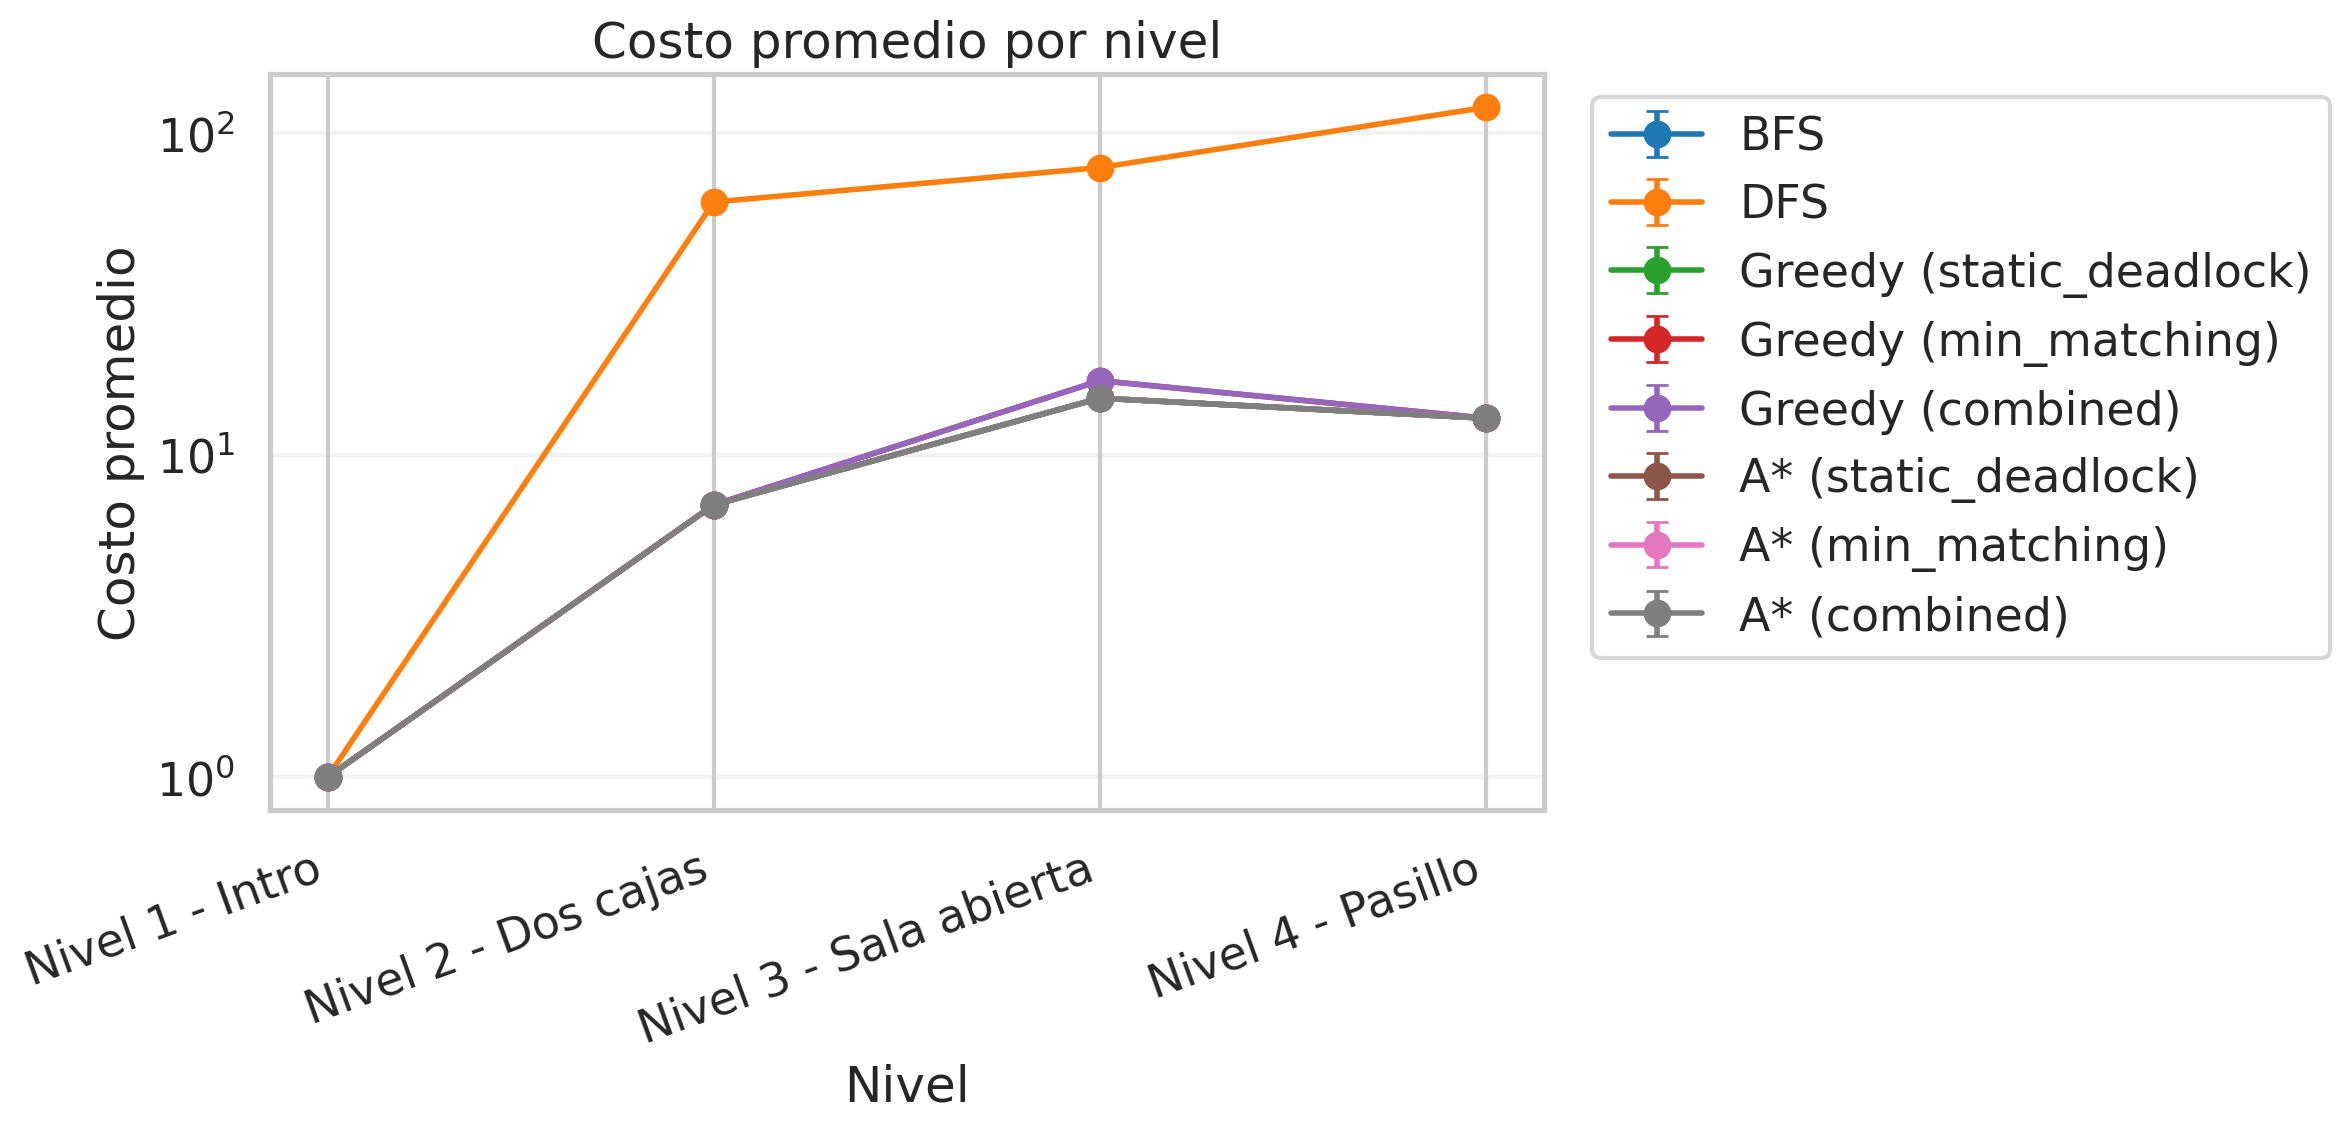
\includegraphics[width=0.82\textwidth]{../results/plots/cost_by_level_errorbars.png}
\end{center}

BFS y A* encuentran la solución óptima en todos los niveles. DFS da costos muy superiores: 61, 78 y 120 donde el óptimo es 7, 15 y 13.

\subsection{Nivel 3 -- Sala abierta (2 cajas, tablero abierto)}

Este es el nivel que mejor muestra las diferencias, porque el branching alto amplifica el efecto de las heurísticas:

\begin{center}
\small
\begin{tabular}{llrrrr}
\toprule
\textbf{Método} & \textbf{Heurística} & \textbf{Costo} & \textbf{Nodos exp.} & \textbf{Frontera} & \textbf{Tiempo} \\
\midrule
BFS     & ninguna          & 15  & 4\,171 & 879 & 26 ms \\
DFS     & ninguna          & 78  & 3\,179 & 75  & 15 ms \\
Greedy  & static\_deadlock & 15  & 680    & 207 & 5 ms \\
Greedy  & min\_matching    & 17  & 47     & 31  & 1 ms \\
Greedy  & combined         & 17  & 47     & 31  & 1 ms \\
A*      & static\_deadlock & 15  & 680    & 125 & 5 ms \\
A*      & min\_matching    & 15  & 133    & 91  & 3 ms \\
A*      & combined         & 15  & 133    & 91  & 3 ms \\
\bottomrule
\end{tabular}
\end{center}

\subsection{Análisis de los resultados}

\textbf{DFS encuentra soluciones mucho peores.} En Nivel 3, DFS da costo 78 cuando el óptimo es 15. En Nivel 4 da 120 vs 13. Esto es esperable: DFS no tiene noción de costo.

\textbf{BFS encuentra el óptimo pero explora más.} BFS expande 4\,171 nodos en Nivel 3 para encontrar costo 15. Es correcto pero costoso.

\textbf{static\_deadlock sola no guía la búsqueda.} A* con static\_deadlock expande los mismos 680 nodos que Greedy con static\_deadlock, porque $h=0$ para estados no muertos. Solo aporta poda binaria ($0$ o $\infty$), sin información numérica.

\textbf{min\_matching es la diferencia clave.} A* con min\_matching baja de 680 a \textbf{133 nodos} --- 5$\times$ menos que con static\_deadlock y 31$\times$ menos que BFS. La heurística da información precisa sobre cuánto falta.

\textbf{combined no mejora sobre min\_matching.} En estos niveles, $\max(\text{matching}, \text{deadlock})$ da los mismos nodos que matching solo. min\_matching ya es consistente, así que A* no necesita reabrir nodos.

\subsection{Gráficos de algoritmos óptimos}

\begin{center}
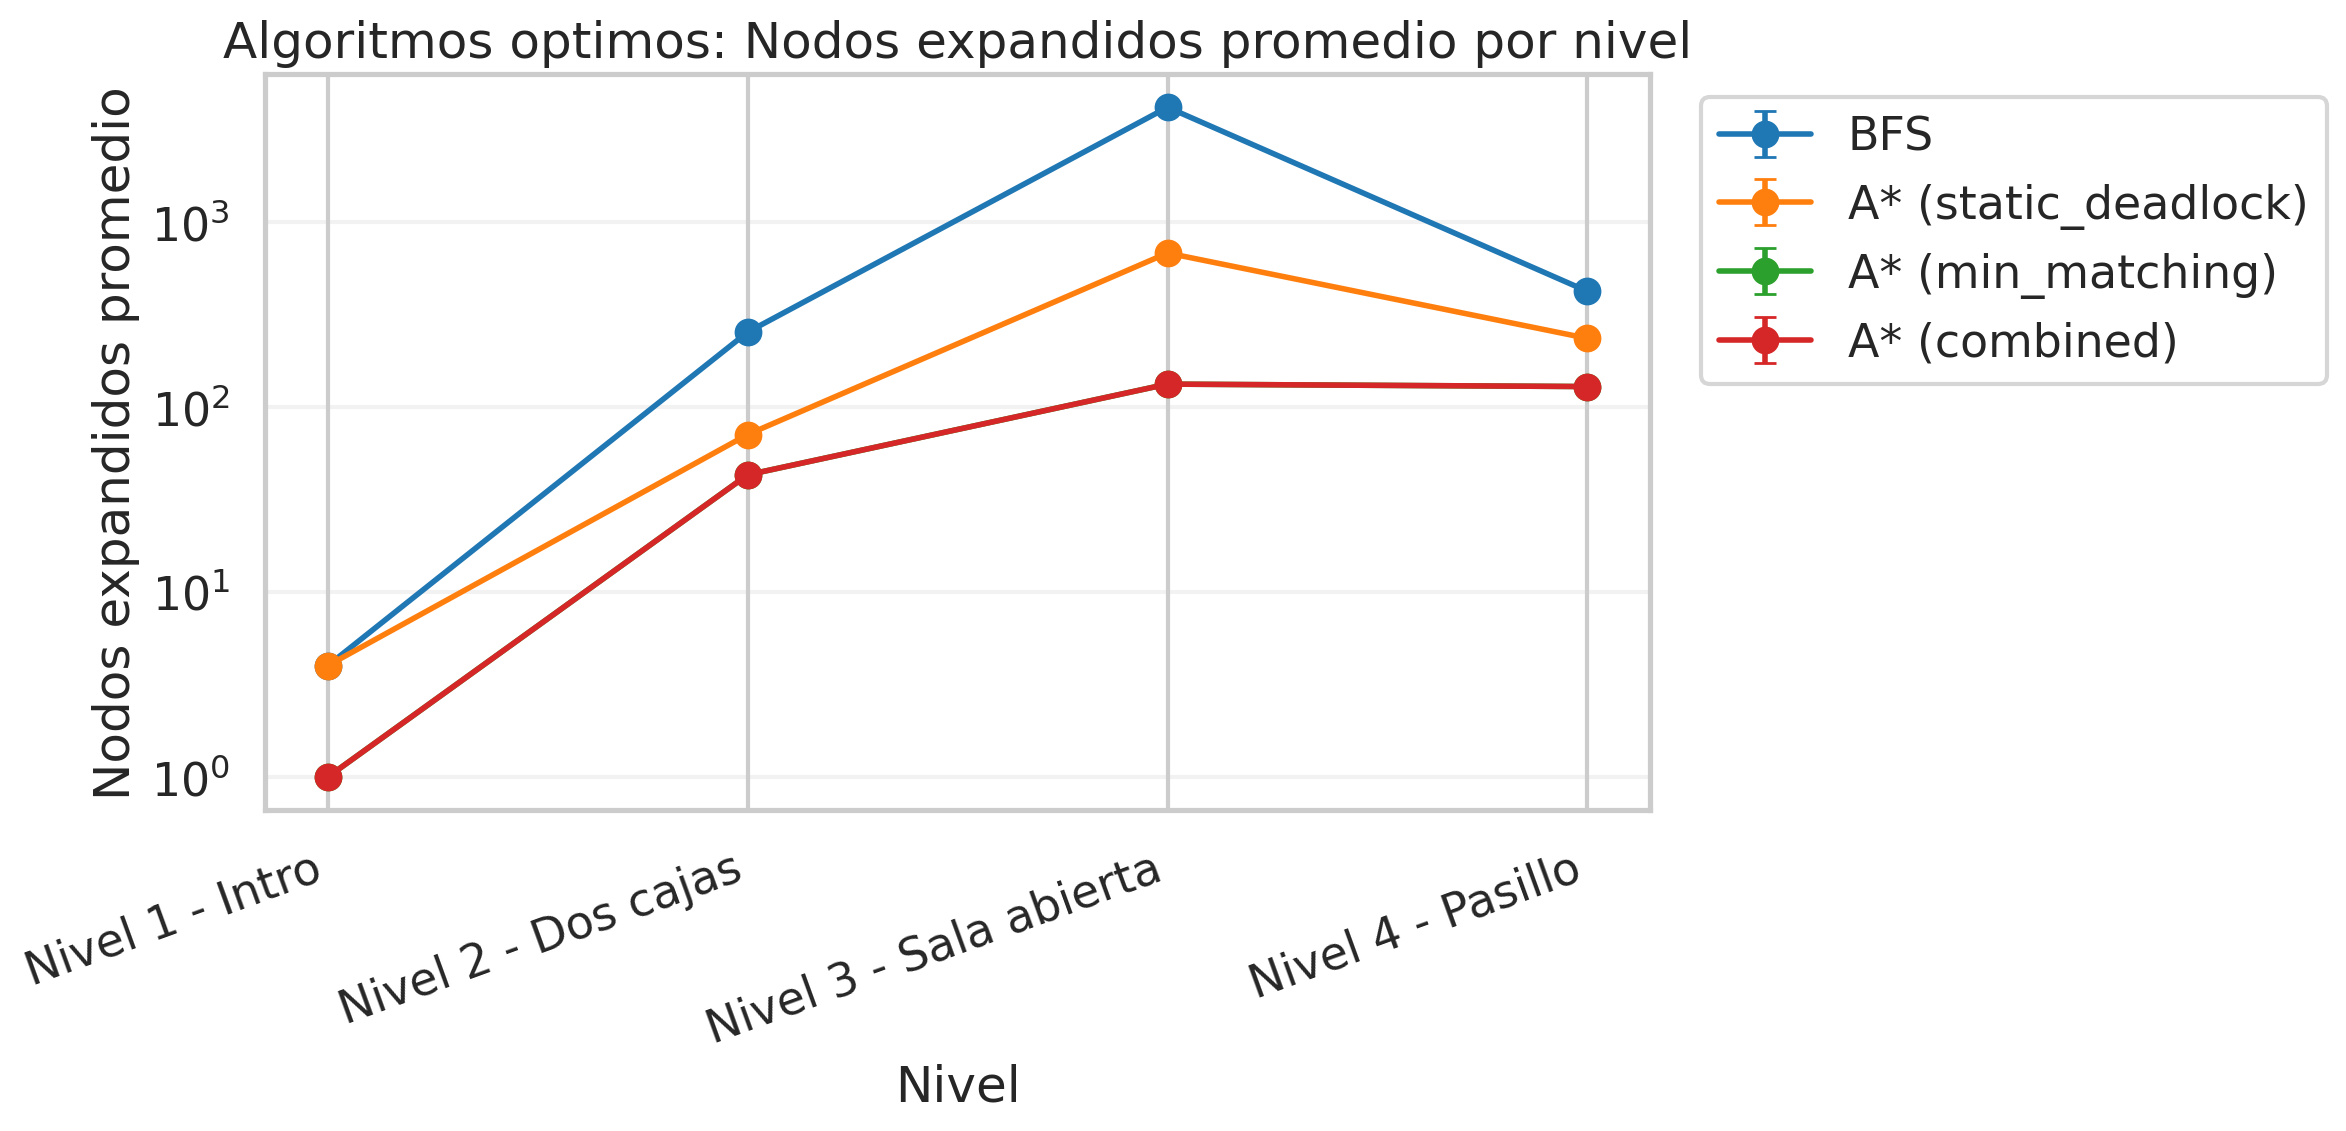
\includegraphics[width=0.82\textwidth]{../results/plots/optimal_nodes_expanded_by_level.png}
\end{center}

\begin{center}
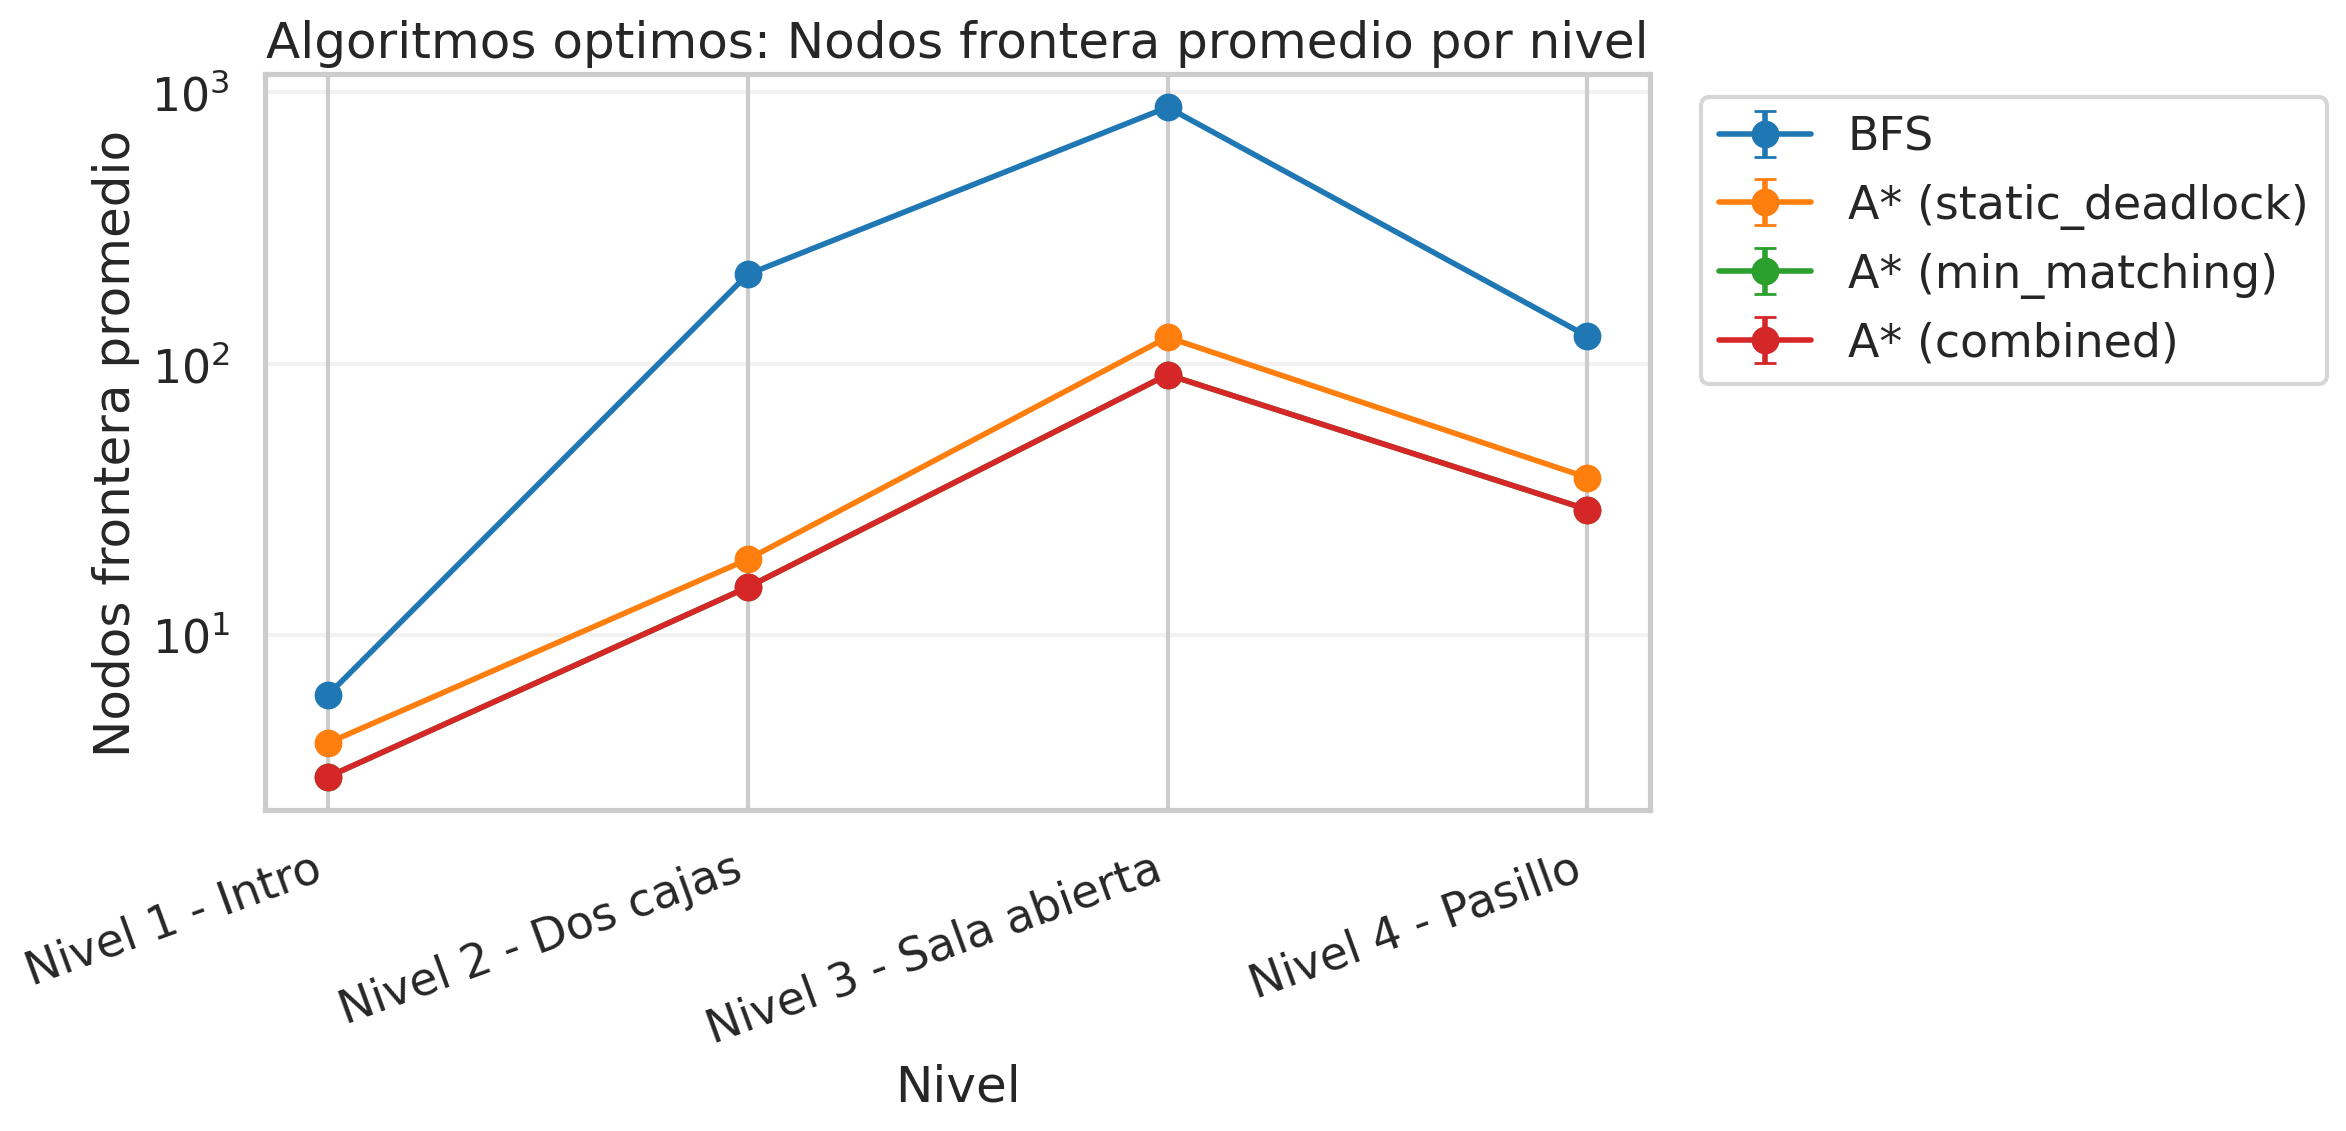
\includegraphics[width=0.82\textwidth]{../results/plots/optimal_frontier_count_by_level.png}
\end{center}

\subsection{Gráficos de algoritmos no óptimos}

\begin{center}
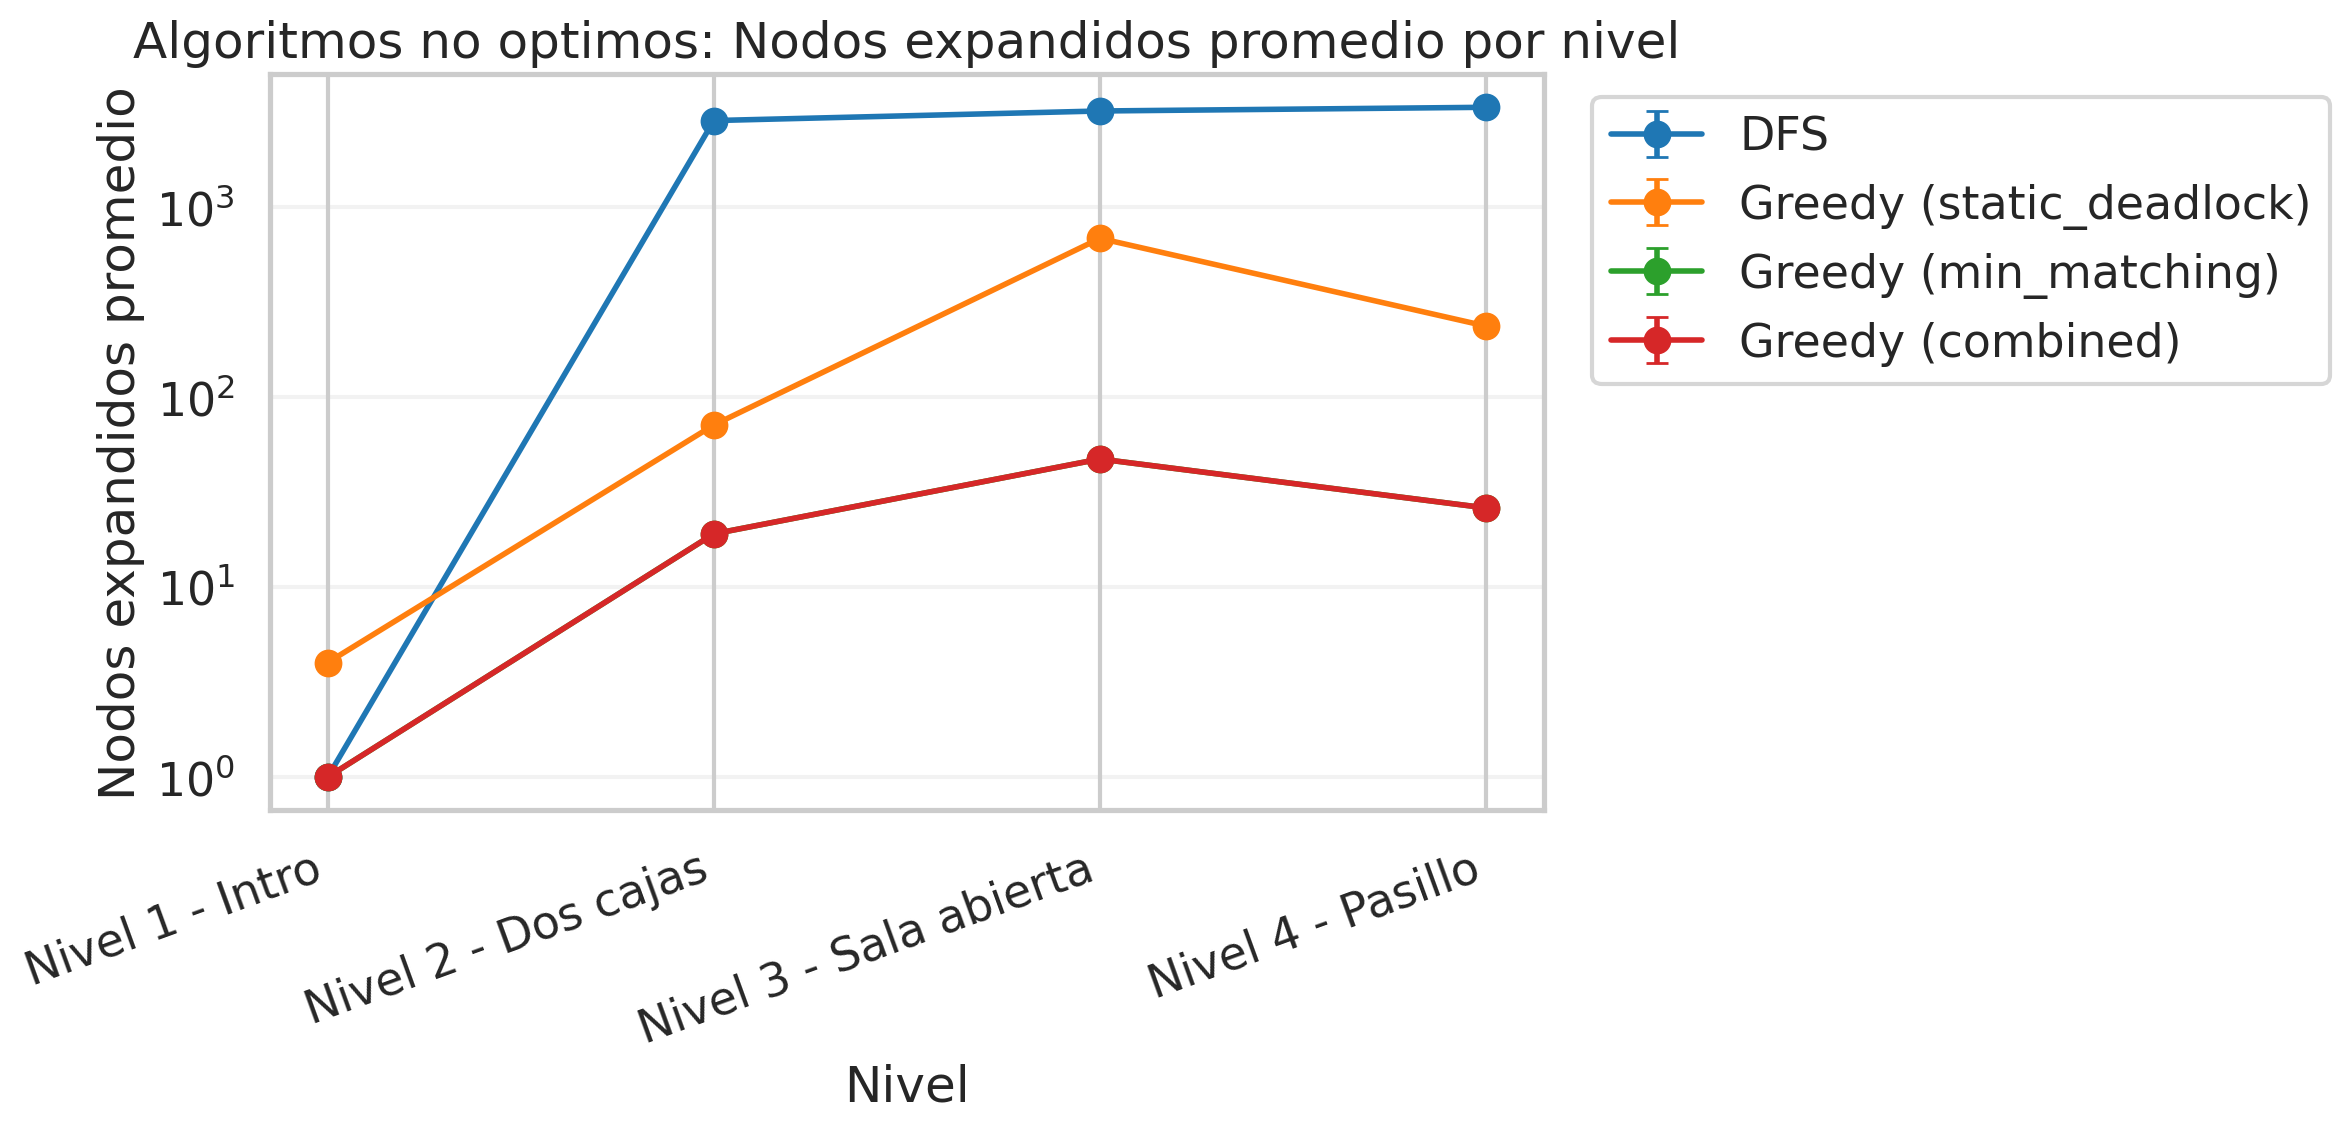
\includegraphics[width=0.82\textwidth]{../results/plots/non_optimal_nodes_expanded_by_level.png}
\end{center}

\subsection{Comparativas directas}

\begin{center}
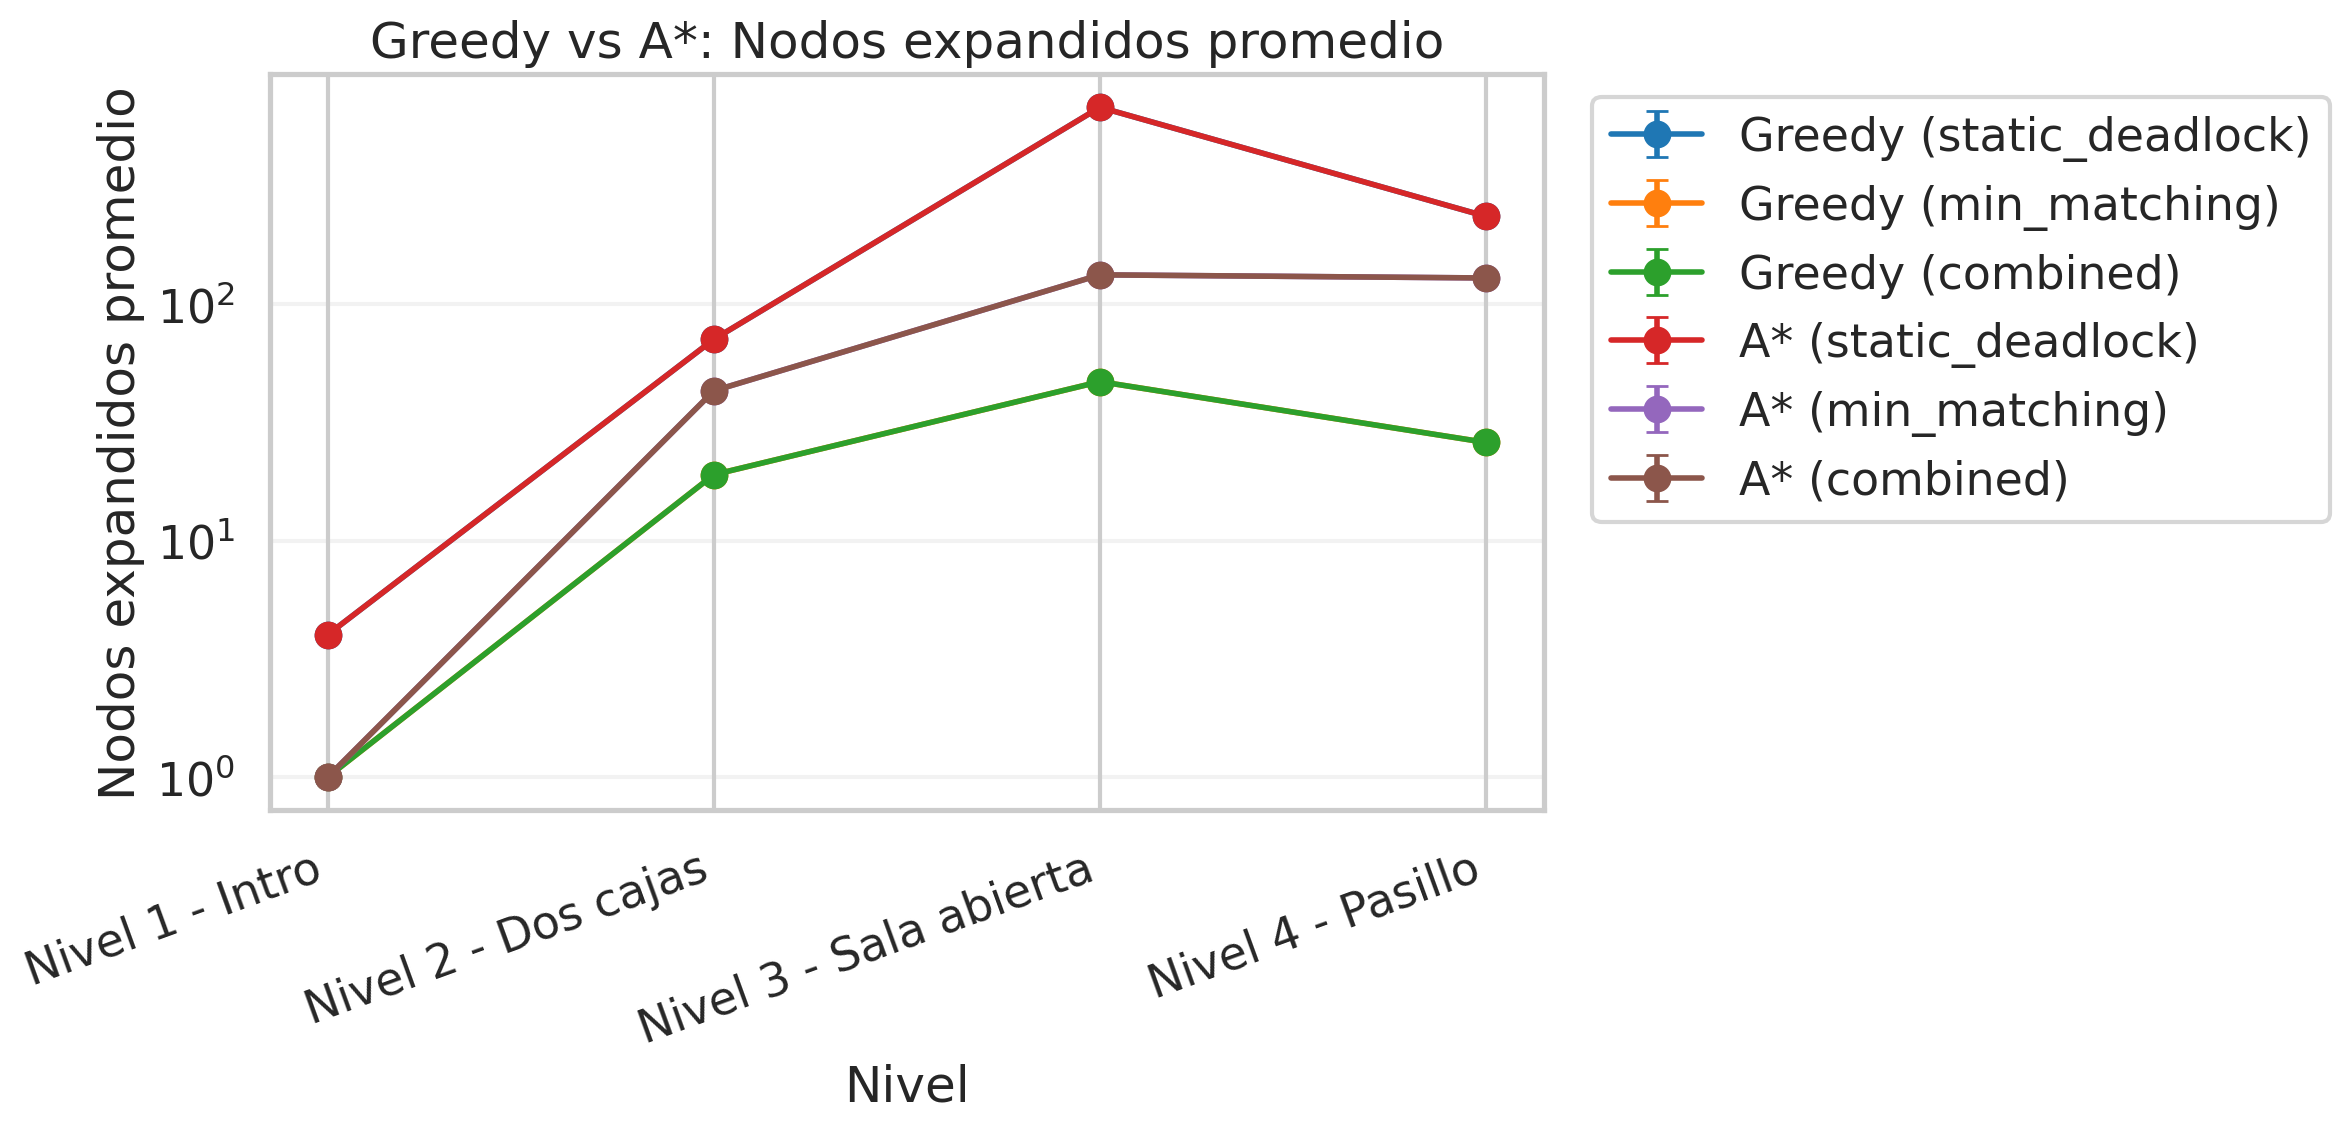
\includegraphics[width=0.82\textwidth]{../results/plots/greedy_vs_astar_nodes_expanded_errorbars.png}
\end{center}

Greedy expande menos nodos (no busca optimalidad) pero A* garantiza costo óptimo. A*(static\_deadlock) expande mucho más porque $h=0$ no guía.

% =============================================================================
\section{Arquitectura del código}
% =============================================================================

\begin{notapresentador}
Esta sección es útil si te piden que expliques la estructura del código o si querés mostrar archivos específicos.
\end{notapresentador}

El proyecto está organizado en módulos:

\begin{itemize}
  \item \texttt{src/model/board\_layout.py}: datos estáticos del tablero (paredes, goals, piso). Se comparte entre estados.
  \item \texttt{src/model/state.py}: la clase \texttt{SokobanState} con la lógica de movimientos y generación de sucesores.
  \item \texttt{src/engine/search.py}: los cuatro algoritmos de búsqueda. Cada uno usa la estructura de datos apropiada (cola, pila, o heap).
  \item \texttt{src/heuristics/static\_deadlocks.py}: BFS inverso para detección de deadlocks estáticos.
  \item \texttt{src/heuristics/min\_matching.py}: asignación mínima con el algoritmo Húngaro.
  \item \texttt{src/heuristics/sokoban\_heuristics.py}: registro de heurísticas, combinación con \texttt{max}, y resolución por nombre.
\end{itemize}

\textbf{Decisiones de diseño clave:}

\begin{enumerate}
  \item \textbf{Inmutabilidad}: usamos \texttt{frozenset} para cajas y goals, lo que permite hashear estados y meterlos en el conjunto de explorados.
  \item \textbf{Cache}: el análisis de deadlocks se computa una vez por layout con \texttt{@lru\_cache}.
  \item \textbf{Separación layout/estado}: el \texttt{BoardLayout} se comparte entre todos los estados, evitando copiar paredes y goals en cada movimiento.
\end{enumerate}

% =============================================================================
\section{Tests}
% =============================================================================

Tenemos 36 tests unitarios en 7 archivos:

\begin{itemize}
  \item \textbf{Tests de A*} (5 tests): reapertura de nodos cerrados, entradas stale en el heap, tie-breaking determinista, cache de heurística, y que A* iguala costo de BFS.
  \item \textbf{Tests de algoritmos} (6 tests): DFS encuentra solución, Greedy encuentra solución, Greedy $\geq$ BFS en costo, estado ya resuelto retorna costo 0, roundtrip de render, guard de recursión en combined.
  \item \textbf{Tests de min\_matching} (9 tests): cajas en goals, shortcircuit una caja, matching óptimo vs greedy, admisibilidad, combinada, A* iguala BFS con min\_matching y combined.
  \item \textbf{Tests de deadlocks} (8 tests): goals no prohibidos, esquinas prohibidas, BFS inverso, poda de sucesores, heurística infinito, combinada, cache por layout.
  \item \textbf{Tests de IO, pipeline y CLI} (8 tests): parser de niveles, runner de benchmarks, policy de deadlocks.
\end{itemize}

Los 36 tests pasan correctamente.

% =============================================================================
\section{Conclusiones}
% =============================================================================

Para cerrar, las conclusiones principales del trabajo:

\begin{enumerate}
  \item \textbf{Las heurísticas informadas reducen drásticamente el espacio explorado.} Pasamos de decenas de miles de nodos con BFS a decenas o cientos con heurísticas informadas. Esto es lo que hace viable resolver puzzles más grandes.

  \item \textbf{No todas las heurísticas son iguales.} La detección de deadlocks es binaria: poda estados imposibles pero no dice cuánto falta. El minimum matching da información numérica que guía la búsqueda mucho más efectivamente.

  \item \textbf{La combinación con max es la forma segura.} Combinar heurísticas con el máximo mantiene la admisibilidad y aprovecha lo mejor de cada una.

  \item \textbf{A* con heurística admisible es el mejor compromiso.} Garantiza optimalidad y, con una buena heurística, explora una fracción del espacio total.

  \item \textbf{El matching óptimo no es trivial.} Como mostramos con el ejemplo concreto, la asignación greedy puede ser subóptima. El algoritmo Húngaro resuelve esto en $O(n^3)$, lo cual es despreciable para la cantidad de cajas típica en Sokoban.
\end{enumerate}

Eso es todo. Quedo a disposición para preguntas.

% =============================================================================
\section*{Apéndice: Preguntas frecuentes de defensa}
% =============================================================================

\begin{notapresentador}
Estas son respuestas preparadas para preguntas típicas que pueden hacer los profesores. No las leés en la presentación, las tenés de backup.
\end{notapresentador}

\textbf{¿Por qué Manhattan y no distancia real?}
Porque la distancia Manhattan es un lower bound de la distancia real (ignora paredes). Eso la hace admisible. Calcular la distancia real requeriría un BFS por cada par caja-goal, lo cual es más costoso computacionalmente.

\textbf{¿Qué pasa si hay más cajas que goals o viceversa?}
En Sokoban estándar siempre coinciden. Nuestro \texttt{is\_goal()} chequea que los conjuntos sean iguales. El matching solo considera cajas fuera de goals y goals vacíos, que siempre tienen la misma cantidad.

\textbf{¿La heurística de deadlocks captura todos los deadlocks?}
No, solo los estáticos. Existen deadlocks dinámicos (como dos cajas trabadas entre sí contra una pared) que requieren un análisis más complejo y no los implementamos. Nuestro análisis es \textit{sound} pero no completo: todo lo que marca como deadlock realmente lo es, pero puede haber deadlocks que no detecta.

\textbf{¿Por qué no implementaron IDDFS?}
Era opcional. IDDFS combina la completitud de BFS con la eficiencia en memoria de DFS usando profundizaciones iterativas. Es útil cuando la memoria es limitada, pero en nuestros niveles de prueba A* con buenas heurísticas es superior.

\textbf{¿Qué pasa con niveles más grandes?}
En niveles con muchas cajas, el espacio de estados crece exponencialmente. Las heurísticas ayudan a podar pero no eliminan la complejidad inherente. Sokoban es PSPACE-complete, así que no hay algoritmo eficiente en el caso general.

\textbf{¿Por qué scipy y no una implementación propia del Húngaro?}
\texttt{scipy.optimize.linear\_sum\_assignment} es una implementación optimizada en C del algoritmo Húngaro. Reimplementarlo en Python puro sería más lento y propenso a bugs. En un contexto académico, es razonable usar bibliotecas establecidas para problemas bien conocidos.

\end{document}
